\section{Experimental Setup}
\label{sec:experiments}
\label{sec:setup}

\paragraph{Intervention implementation.}
All inference-time edits operate strictly during the forward pass and leave
model weights untouched. We apply component scaling across decoder layers in
two distinct sites: the residual stream and attention value space.
In value space, we explicitly evaluate both \textit{full-aggregate} scaling
(decomposing the complete attention aggregate $\mathbf{o}_t$ relative to $\mathbf{v}_t$)
and \textit{exclude-self} scaling (Equation~\ref{eq:exclude-self-scaling}).
Because the query token's direct self message $\mathbf{d}_t = \Adiag{t}\mathbf{v}_t$
is intrinsically parallel to $\mathbf{v}_t$, naive parallel removal on the full
aggregate inadvertently suppresses the token's primary identity carrier along with
cross-token updates, causing severe degradation (Section~\ref{sec:value-vs-residual-exp}).
Exclude-self scaling preserves $\mathbf{d}_t$ to isolate whether cross-token contextual
magnitude modulation is truly redundant. Unless explicitly marked otherwise,
value-space evaluations use exclude-self scaling.
Appendices~\ref{app:evaluation-details} and~\ref{app:method} provide complete
evaluation and implementation details.

\paragraph{Models and benchmarks.}
We evaluate across dense and mixture-of-experts architectures from the
Qwen3~\citep{Yang2025Qwen3TR}, Llama-3~\citep{Dubey2024TheL3}, and
Gemma-3~\citep{GemmaTeam2025Gemma3} families across scales up to 30B parameters.
Our benchmarks include language modeling perplexity, seven standard zero-shot
commonsense and reasoning tasks, long-context retrieval and reasoning (13-task
RULER suite~\citep{Hsieh2024RULERWT} up to 12k context lengths), and
post-training compression under 4-bit AWQ~\citep{Lin2023AWQAW} and Wanda
pruning~\citep{Sun2023ASA} (unstructured, 4:8, and 2:4).

\paragraph{Pretraining setup.}
For training-time investigations, we pretrain GPT-style models from scratch on
OpenWebText~\citep{Gokaslan2019OpenWeb} across scales from 296M to 2.7B parameters,
comparing baseline optimization against residual- and value-space
parallel removal; Appendix~\ref{app:training-configs} details architectural
configurations and training hyperparameters.

% ------------------------------------------------------------------
\section{Inference-Time Component Editing}
\label{sec:editing-diagnostics}

\subsection{Directional Component Scaling}
\label{sec:zeroshot}

\paragraph{Probing directional sensitivity.}
Section~\ref{sec:method} formalized the orthogonal decomposition into parallel
magnitude modulation and perpendicular semantic steering across residual and
value spaces. We first evaluate the functional roles of these components by
measuring model sensitivity to continuous inference-time scaling edits.
Holding weights frozen, Figure~\ref{fig:residual-component-editing} independently
varies $s^{(\parallel)}$ (left, $s^{(\perp)}=1$) and $s^{(\perp)}$ (right,
$s^{(\parallel)}=1$) across three intervention sites on Qwen3-1.7B:
value space (exclude-self), residual attention, and residual MLP.

\paragraph{Directional asymmetry: acute perpendicular fragility.}
Across all three intervention sites, model behavior exhibits an acute
\textit{directional asymmetry}. Perpendicular scaling ($s^{(\perp)} \ne 1$)
proves extraordinarily hyper-fragile: even minor deviations from identity
immediately destabilize the model with steep perplexity surges, while severe
attenuation or complete removal ($s^{(\perp)}=0$) triggers catastrophic
breakdown, escalating by multiple orders of magnitude across all sites (reaching
tens of thousands of points in value space and residual attention, and exploding
into millions of points in residual MLP). This confirms that orthogonal
directions govern delicate, non-interchangeable semantic steering. In stark
contrast, parallel scaling ($s^{(\parallel)}$) displays a broad, stable tolerance
basin, confirming parallel updates regulate representation magnitude
rather than categorical semantic trajectories.

\paragraph{Site asymmetry: value space vs.\ residual branches.}
Within the parallel axis, the sweeps reveal a pronounced \textit{site
hierarchy}. Value-space manipulation (with the direct self message preserved)
stays closest to baseline, remaining virtually flat across
$s^{(\parallel)} \in [0, 1]$ (shifting PPL by less than a point, and by at most
1.3 points up to scale 3). In the residual stream, Residual(Attn) is
intermediate, whereas Residual(MLP) is most fragile, collapsing rapidly
outside the unit interval.

This hierarchy demonstrates that robustness is not an inherent property of
``parallelness'' in the abstract, but depends decisively on representation space
and what is preserved. Residual-space parallel edits modify the accumulated
features of the main stream, where parallel updates carry essential cross-layer
computation. In contrast, value-space exclude-self editing modulates only
cross-token contextual aggregation while leaving the query token's primary
identity carrier ($\mathbf{d}_t = \Adiag{t}\mathbf{v}_t$) and perpendicular context
intact. A parallel effect appears inside the MLP: decomposing the internal
post-gating carrier rather than the final sub-layer output similarly preserves
performance under parallel removal (Appendix~\ref{app:mlp-internal-carrier}).

\subsection{Cross-Space Representation Editing}
\label{sec:value-vs-residual-exp}

\paragraph{Robustness on general tasks.}
We evaluate downstream zero-shot robustness across seven standard benchmarks on
dense (Qwen3-1.7B) and MoE (Qwen3-30B-A3B) models (Table~\ref{tab:general-zeroshot}),
comparing three primary approaches: (1) self-preserving value-space removal
(V-Excl.-self), (2) naive full-aggregate value removal (V-Para Rem.), and (3)
residual-space and diagonal controls (Attn Para-Rem.\ and Diag.\ Rem.).

When parallel removal is applied naively to the entire value aggregate (V-Para Rem.),
average performance drops by 8--10 points across both models. This degradation
illustrates why isolating self-attention is essential: naive value-space editing
suppresses the token's own identity carrier $\Adiag{t}\mathbf{v}_t$ alongside
cross-token messages, inadvertently disrupting representation propagation.

In stark contrast, preserving the direct self-message while scaling only
cross-token aggregation (V-Excl.-self) leaves performance virtually intact across
all seven benchmarks—trailing baseline by only 1.5 points on 1.7B and virtually
matching it on the 30B-A3B MoE model (within 0.1 points), with slight gains on
several individual tasks. Meanwhile, residual-space attention removal (Attn
Para-Rem.) incurs steady drops across tasks, and hard diagonal removal (Diag.\ Rem.)
severely degrades the models because forcing $\Adiag{t}=0$ artificially renormalizes
attention weights over off-diagonal positions. Together, these comparisons
establish that cross-token parallel updates are functionally redundant, provided
direct self-representations are retained.

\begin{table*}[t]
  \caption{\textbf{Task-level comparison of residual-, value-space, and diagonal controls.}
  Entries are absolute scores (\%); higher is better and Avg. is unweighted.
  Both value-space rows set $s_{\parallel}=0$. V-Para Rem. edits the full
  value aggregate; V-Excl.-self preserves $\Adiag{t}\mathbf{v}_t$. Diag.\ Rem.\
  zeros $\Adiag{t}$ and renormalizes over non-self positions.
  Attn Para-Rem.\ and Diag.\ Rem.\ use separate matched
  baselines. Differences reported in the text are computed before rounding.
  Bold marks the best baseline/value-space result.}
  \label{tab:general-zeroshot}
  \centering
  \scriptsize
  \setlength{\tabcolsep}{3.1pt}
  \resizebox{\textwidth}{!}{%
  \begin{tabular}{llrrrrrrrr}
    \toprule
    Model & Setting & OBQA & PIQA & Wino & ARC-C & HSwag & BoolQ & RTE & \underline{Avg.} \\
    \midrule
    \multirow{5}{*}{Qwen3-1.7B}
      & Baseline & 37.20 & \textbf{72.47} & \textbf{60.69} & \textbf{53.07} & \textbf{60.16} & \textbf{77.65} & \textbf{70.04} & \underline{\textbf{61.61}} \\
      & Attn Para-Rem. & 38.20 & 72.31 & 56.59 & 50.09 & 58.74 & 71.38 & 66.79 & \underline{59.16} \\
      & V-Para Rem. & 34.40 & 69.48 & 54.85 & 41.38 & 54.04 & 66.27 & 53.43 & \underline{53.41} \\
      & V-Excl.-self & \textbf{39.20} & 71.76 & 60.54 & 49.15 & 59.88 & 74.46 & 65.70 & \underline{60.10} \\
      & Diag. Rem. & 26.20 & 51.36 & 49.17 & 24.49 & 26.66 & 40.70 & 55.60 & \underline{39.17} \\
    \midrule
    \multirow{5}{*}{Qwen3-30B-A3B}
      & Baseline & \textbf{44.80} & \textbf{80.69} & 70.24 & \textbf{69.97} & 77.79 & \textbf{88.53} & 81.95 & \underline{\textbf{73.42}} \\
      & Attn Para-Rem. & 44.00 & 78.73 & 66.85 & 65.10 & 73.87 & 88.04 & 78.34 & \underline{70.70} \\
      & V-Para Rem. & 41.20 & 76.22 & 64.56 & 59.04 & 69.57 & 70.89 & 62.45 & \underline{63.42} \\
      & V-Excl.-self & 44.60 & 79.87 & \textbf{72.45} & 68.34 & \textbf{78.13} & 86.36 & \textbf{83.39} & \underline{73.31} \\
      & Diag. Rem. & 30.60 & 57.67 & 48.46 & 26.96 & 34.78 & 38.59 & 47.65 & \underline{40.68} \\
    \bottomrule
  \end{tabular}
  }
\end{table*}

\paragraph{Context-length scalability.}
Table~\ref{tab:longcontext-ruler} reinforces this distinction as context expands
(RULER on Llama-3.2-3B from 4k to 12k). Retaining half of the parallel component
($\spara=0.5$) with the self-message fixed closely tracks the unedited baseline
across all sequence lengths (within 0.2 points at 4k and 2.4 points at 12k),
consistently outperforming full-aggregate scaling. Under complete removal
($\spara=0$), full-aggregate editing collapses by 26--40 points, whereas
exclude-self retains over $75\%$ accuracy at 4k and maintains substantially higher
resilience out to 12k. Table~\ref{tab:appendix-ruler-full} in the Appendix
details 13-task breakdowns and multi-model evaluations.

\begin{table}[!htbp]
  \caption{\textbf{Long-context performance across sequence lengths.}
  Reported scores are mean accuracy (\%) across all 13 RULER tasks on
  Llama-3.2-3B for context lengths from 4k to 12k tokens. V-Full scales
  the entire value aggregate; V-Excl.-self preserves direct self messages
  $\mathbf{d}_t$ and scales only cross-token context.}
  \label{tab:longcontext-ruler}
  \centering
  \footnotesize
  \renewcommand{\arraystretch}{0.95}
  \begin{tabular*}{\linewidth}{@{\extracolsep{\fill}}lcrrr}
    \toprule
    Method & $s_\parallel$ & 4k & 8k & 12k \\
    \midrule
    Baseline & $1.0$ & 86.91 & 82.09 & 79.30 \\
    V-Full & $0.5$ & 84.81 & 78.80 & 74.76 \\
    V-Excl.-self & $0.5$ & \textbf{86.69} & \textbf{80.80} & \textbf{76.88} \\
    V-Full & $0.0$ & 60.99 & 48.61 & 39.17 \\
    V-Excl.-self & $0.0$ & 75.64 & 67.97 & 62.02 \\
    \bottomrule
  \end{tabular*}
\end{table}

\paragraph{Attention diagonal views for parallel editing.}
\label{sec:diagonal-validation}
All three attention-side interventions admit closed-form expressions as effective
diagonal modifications on the attention matrix (Section~\ref{sec:closed-form-control}).
Figure~\ref{fig:attn-maps} compares the empirical attention map of Qwen3-4B
(layer 19, head 6) under baseline against the residual-space and value-space
diagonal views (see Table~\ref{tab:effective-diagonal-derivation} in the Appendix
for complete mathematical derivations).

\begin{figure}[tb]
  \centering
  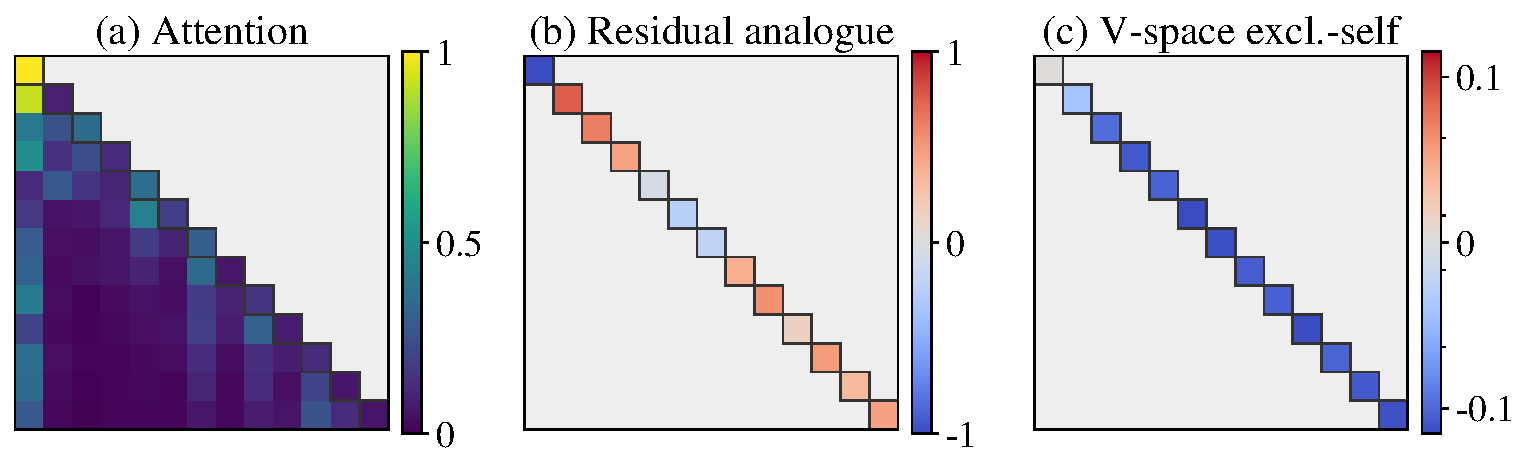
\includegraphics[width=0.97\linewidth]{figs/attn_matrix_corrected/qwen3-4b/layer19/h6_diag_delta_corrected_titles.pdf}
  \caption{\textbf{Attention diagonal views of parallel editing.}
  For full parallel removal ($s_{\parallel}=0$), the left panel shows empirical
  attention weights (Qwen3-4B, layer 19, head 6); the middle shows the residual-space
  attention-map view, and the right shows the exclude-self value-space change.
  The latter two color scales encode $\Delta A_{tt}$; off-diagonal entries are unchanged.}
  \label{fig:attn-maps}
\end{figure}

The residual-space diagonal view induces volatile positive and negative adjustments
(spanning $-1.00$ to $0.76$), whereas exclude-self value-space editing preserves
direct self-token routing with bounded, non-positive diagonal shifts.
Crucially, this localized stability does not mean value-space editing is gentler:
auditing the post-$W_O$ attention output on Qwen3-0.6B reveals
that removing parallel context across non-self tokens induces a much larger
perturbation norm than residual-space removal ($49.10\%$ versus $25.15\%$ of
unedited branch norm; Table~\ref{tab:applied-no-para-strength}).
That value-space editing preserves model capabilities despite altering attention
outputs nearly twice as much proves that stability is governed by preserving
self-identity routing and residual propagation trajectories, rather than minimizing
isotropic perturbation magnitude.
Appendix~\ref{app:head-localization} details head-level localization.

% ------------------------------------------------------------------
\subsection{Compression Diagnostics}
\label{sec:compression-error-geometry}

% Declare the double-column training figure before the single-column
% compression figure so it can occupy the top of the following page without
% terminating that page after the first column.
\begin{figure*}[t]
  \centering
  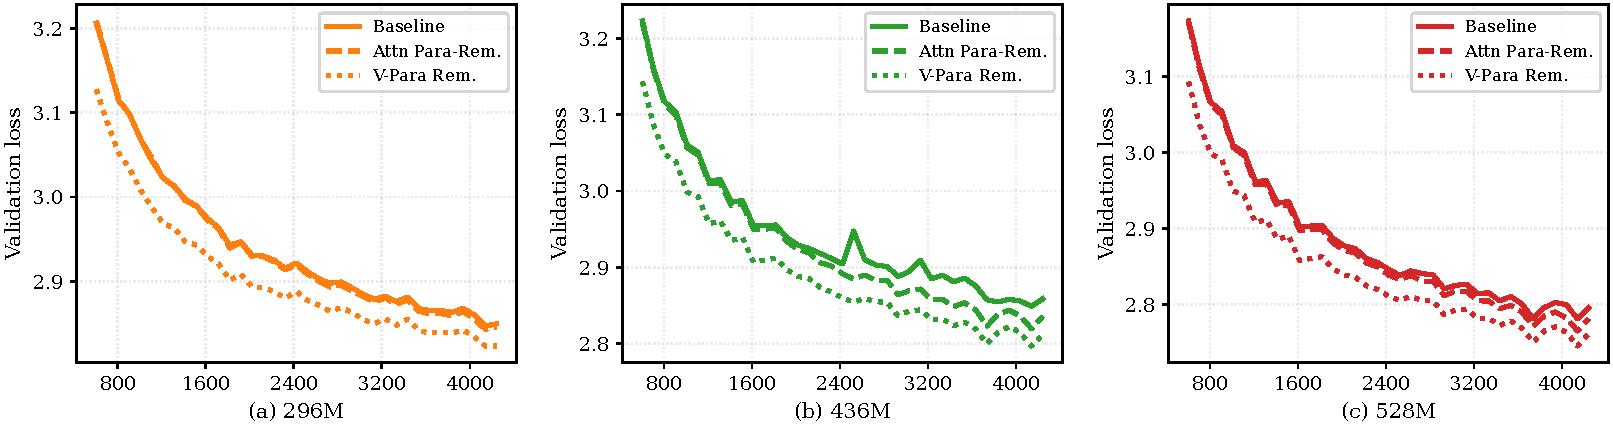
\includegraphics[width=0.84\textwidth]{figs/loss_curves_corrected/pretraining_loss_by_size_restored.pdf}
  \caption{\textbf{Training-time parallel removal lowers validation loss.}
  The displayed OpenWebText~\citep{Gokaslan2019OpenWeb} loss trajectories
  show baseline, Attn Para-Rem., and V-Para Rem. for matched configurations across
  296M, 436M, and 528M model sizes. Both interventions set $\spara=0$ and retain
  the perpendicular component.}
  \label{fig:pretraining}
  \vspace{-0.8em}
\end{figure*}

The removal experiments establish that model capabilities are exceptionally
sensitive to direction-changing components of activation updates. We next ask
how this geometric principle manifests under post-training compression. Compression
alters model parameters, inducing an error between uncompressed and compressed
updates rather than an explicit activation edit. Decomposing this error into
parallel and perpendicular components provides a principled test: if orthogonal
steering is the behaviorally critical component, superior compression algorithms
should systematically exhibit lower perpendicular distortion, whereas parallel error
should be far less diagnostic.

Concretely, at each layer, let $\Delta_{\mathrm{base}}$ denote the uncompressed
baseline update and $\Delta_{\mathrm{comp}}$ denote the compressed update. The local
compression error is $e = \Delta_{\mathrm{comp}} - \Delta_{\mathrm{base}}$. We
decompose $e$ relative to the baseline update direction:
$e_{\parallel} = \mathrm{proj}_{\Delta_{\mathrm{base}}} e$ and
$e_{\perp} = e - e_{\parallel}$. Figure~\ref{fig:local-flip-attn} reports the
normalized component norms $\|e_{\perp}\|/\|\Delta_{\mathrm{base}}\|$ and
$\|e_{\parallel}\|/\|\Delta_{\mathrm{base}}\|$ across layers of Qwen3-4B under
4-bit AWQ and 50\% Wanda pruning (unstructured, 4:8, and 2:4).

\begin{figure}[t]
  \centering
  
\includegraphics[width=0.80\linewidth]{figs/comp_analysis/local_flip_compare-attn_out-perp_over_base_update.pdf}\par
  {\small (a) Perpendicular attention-output error.\par}

  \vspace{0em}
  
\includegraphics[width=0.80\linewidth]{figs/comp_analysis/local_flip_compare-attn_out-para_over_base_update.pdf}\par
  {\small (b) Parallel attention-output error.\par}
  \caption{\textbf{Directional decomposition of compression error.}
  Curves are layerwise means, with bands showing one standard deviation over 12 fixed prompts,
  comparing compressed and baseline Qwen3-4B attention updates. The upper and
  lower panels show perpendicular and parallel error, each normalized by the
  full baseline-update norm (higher is more distortion). Settings are
  4-bit AWQ and 50\% Wanda pruning with unstructured, 4:8, or 2:4 masks.}
  \label{fig:local-flip-attn}
  \vspace{-1em}
\end{figure}

The results strongly corroborate this directional hypothesis: perpendicular error
curves cleanly separate the four compression regimes in strict alignment with their
downstream fidelity (4-bit AWQ achieves the lowest error, followed by unstructured,
4:8, and 2:4 Wanda). In contrast, parallel error curves heavily interleave and fail
to provide a consistent ranking. This clarifies why conventional isotropic $L_2$ error
can fail to predict degradation: isotropic distance conflates benign magnitude shifts
with disruptive semantic rotations. Appendix~\ref{app:compression} substantiates
this mechanism across the MLP branch and full block updates, showing that perpendicular
distortion dominates total compression error ($r > 0.97$, Table~\ref{tab:local-total-perp-alignment})
and connecting this geometry to cosine-based pruning diagnostics.

% ------------------------------------------------------------------
\section{Training-Time Allocation}
\label{sec:pretraining}

In standard Transformer pretraining, attention updates conflate colinear magnitude
rescaling with orthogonal contextual steering. \textit{We investigate whether suppressing
parallel attention updates throughout training shifts how optimization allocates
representational capacity across direction-changing components.} We train GPT-style
language models from scratch on standard next-token prediction, enforcing parallel
removal during both optimization and evaluation to eliminate train--evaluation mismatch.
We evaluate these interventions through validation trajectories and downstream
benchmarks; Appendix~\ref{app:training-configs} gives model configurations and
gated-scaling controls.

Figure~\ref{fig:pretraining} plots OpenWebText~\citep{Gokaslan2019OpenWeb} validation loss
trajectories across model sizes (296M, 436M, and 528M). Suppressing parallel
attention updates shifts the learning trajectory downward from early training
stages, and this advantage persists consistently through the final checkpoint
rather than emerging only as an endpoint artifact.

Table~\ref{tab:pretraining-summary} reports downstream zero-shot accuracy across
six standard benchmarks for the scaled 1.4B and 2.7B models. Both interventions
improve downstream performance over the baseline at both scales, with value-space
parallel removal achieving the largest gains ($+0.7$ points on 1.4B and $+1.5$ points on 2.7B).
Together with training trajectories, these findings demonstrate that
directional decomposition provides an effective inductive bias: suppressing
parallel updates directs attention capacity toward orthogonal contextual steering,
improving downstream generalization.

\begin{table}[t]
  \caption{\textbf{Downstream generalization across model scales.}
  Unweighted mean accuracy over six benchmarks (ARC-Easy, BoolQ, HellaSwag,
  OpenBookQA, PIQA, WinoGrande); \(\Delta\)Avg is relative to matched baseline.
  Attn and V-Para denote residual and value parallel removal.}
  \label{tab:pretraining-summary}
  \centering
  \small
  \renewcommand{\arraystretch}{0.96}
  \begin{tabular*}{0.92\columnwidth}{@{\extracolsep{\fill}}llrr}
    \toprule
    Model & Setting & Avg & $\Delta$Avg \\
    \midrule
    \multirow{3}{*}{1.4B}
      & Baseline & 58.5 & 0.0 \\
      & Attn Para-Rem. & 58.8 & +0.3 \\
      & V-Para Rem. & \textbf{59.2} & \textbf{+0.7} \\
    \midrule
    \multirow{3}{*}{2.7B}
      & Baseline & 60.2 & 0.0 \\
      & Attn Para-Rem. & 60.9 & +0.7 \\
      & V-Para Rem. & \textbf{61.7} & \textbf{+1.5} \\
    \bottomrule
  \end{tabular*}
\end{table}

Appendix~\ref{app:training-configs} details task-level scores for both larger
models and the gated-scaling control, where fixed removal maintains the lowest
training loss.
